\def\year{2015}
%File: formatting-instruction.tex
\documentclass[letterpaper]{article}
\usepackage{aaai}
\usepackage{times}
\usepackage{helvet}
\usepackage{courier}
%%
\usepackage{graphicx}
\usepackage{url}
\usepackage{amsfonts}
\usepackage{moreverb}
%%
\usepackage{bm}
\usepackage{paralist}
%\usepackage{minted}
%%
% so we don't need to specify figures subdirectory in figure code
\graphicspath{{./figures/}}
\usepackage{subfig}
%needed to change table colors
\usepackage[table]{xcolor}

%%
\frenchspacing
\setlength{\pdfpagewidth}{8.5in}
\setlength{\pdfpageheight}{11in}
\pdfinfo{
/Title (Insert Your Title Here)
/Author (Put All Your Authors Here, Separated by Commas)}
\setcounter{secnumdepth}{0}  
 \begin{document}
% The file aaai.sty is the style file for AAAI Press 
% proceedings, working notes, and technical reports.
%
\title{Activity Monitoring and Prediction for Humans and NAO Humanoid Robots using 
Wearable Sensors}
% \author{Author names \\ %Saminda Abeyruwan \and Faisal Sikder \and Dilip Sarkar\\
% University of Miami \\
% Department of Computer Science\\
% 1365 Memorial Drive, Coral Gables, FL, 33146, USA\\
% %{\ttfamily \{saminda|f.sikder|sarkar\}@cs.miami.edu}
% }
\maketitle
\begin{abstract}
\begin{quote}
Monitoring and learning from activities such as jogging, running, falling so forth for humans and 
humanoid biped robots provide predictions to improve the activities as well as to prevent 
accidental or unforeseen situations. The predictions must be delivered within the time scales of 
the activities for gain maximum performance. In order to learn from activities and to provide 
predictions, the two demographic groups are impel to ware external devices with sensors. This 
paper provides: \begin{inparaenum}[1)] \item a generalize method to learn and predict activities 
of the groups; and \item a modular software framework to realize learning/predictions 
efficiently on embedded devices. \end{inparaenum} We have use on/off-line reactive and deliberative 
methods to learn from activities and to provide predictions. Our software development platform has 
been tested on MSP-EXP430G2, Tiva C Series EK-TM4C123GXL, and Tiva C Series TM4C129 Connected 
LaunchPads. It is lightweight, flexible, and consumes minimum memory and computational 
resources to develop applications and rational agents on microcontrollers that sense and actuate 
using add-on boards. We have used our framework to learn from activities and to deliver predictions 
on able-bodied humans and on NAO biped humanoid robots. We empirically evaluate the outcomes and 
show the success of the methods on different activity settings. 
\end{quote}
\end{abstract}

\section{Introduction}

The humans as well as the biped humanoid robots complete tasks with complex activities. These 
activities include jogging, running, falling so forth. Some of these activities are 
considered safe, while, others such as falling abruptly would cause damage to human body 
or to the structural components of a humanoid robot \cite{li2009accurate}. There has been an 
increasing demand in domains such as rescue to use autonomous or teleoperated humanoid robots to 
complete high-risk tasks otherwise would have been lethal to a human subject. Therefore, we 
hypotheses environments where humans and humanoid robots collaboratively work to complete 
tasks. We also hypotheses that learned prediction of activities in both groups can be 
generalizable. This paper is a step towards that direction to use wearable devices with sensor to 
learn, predict, and generalize across the two demographic groups.

\begin{figure*}[!t]
\centering
\subfloat[]{\label{fig:fa}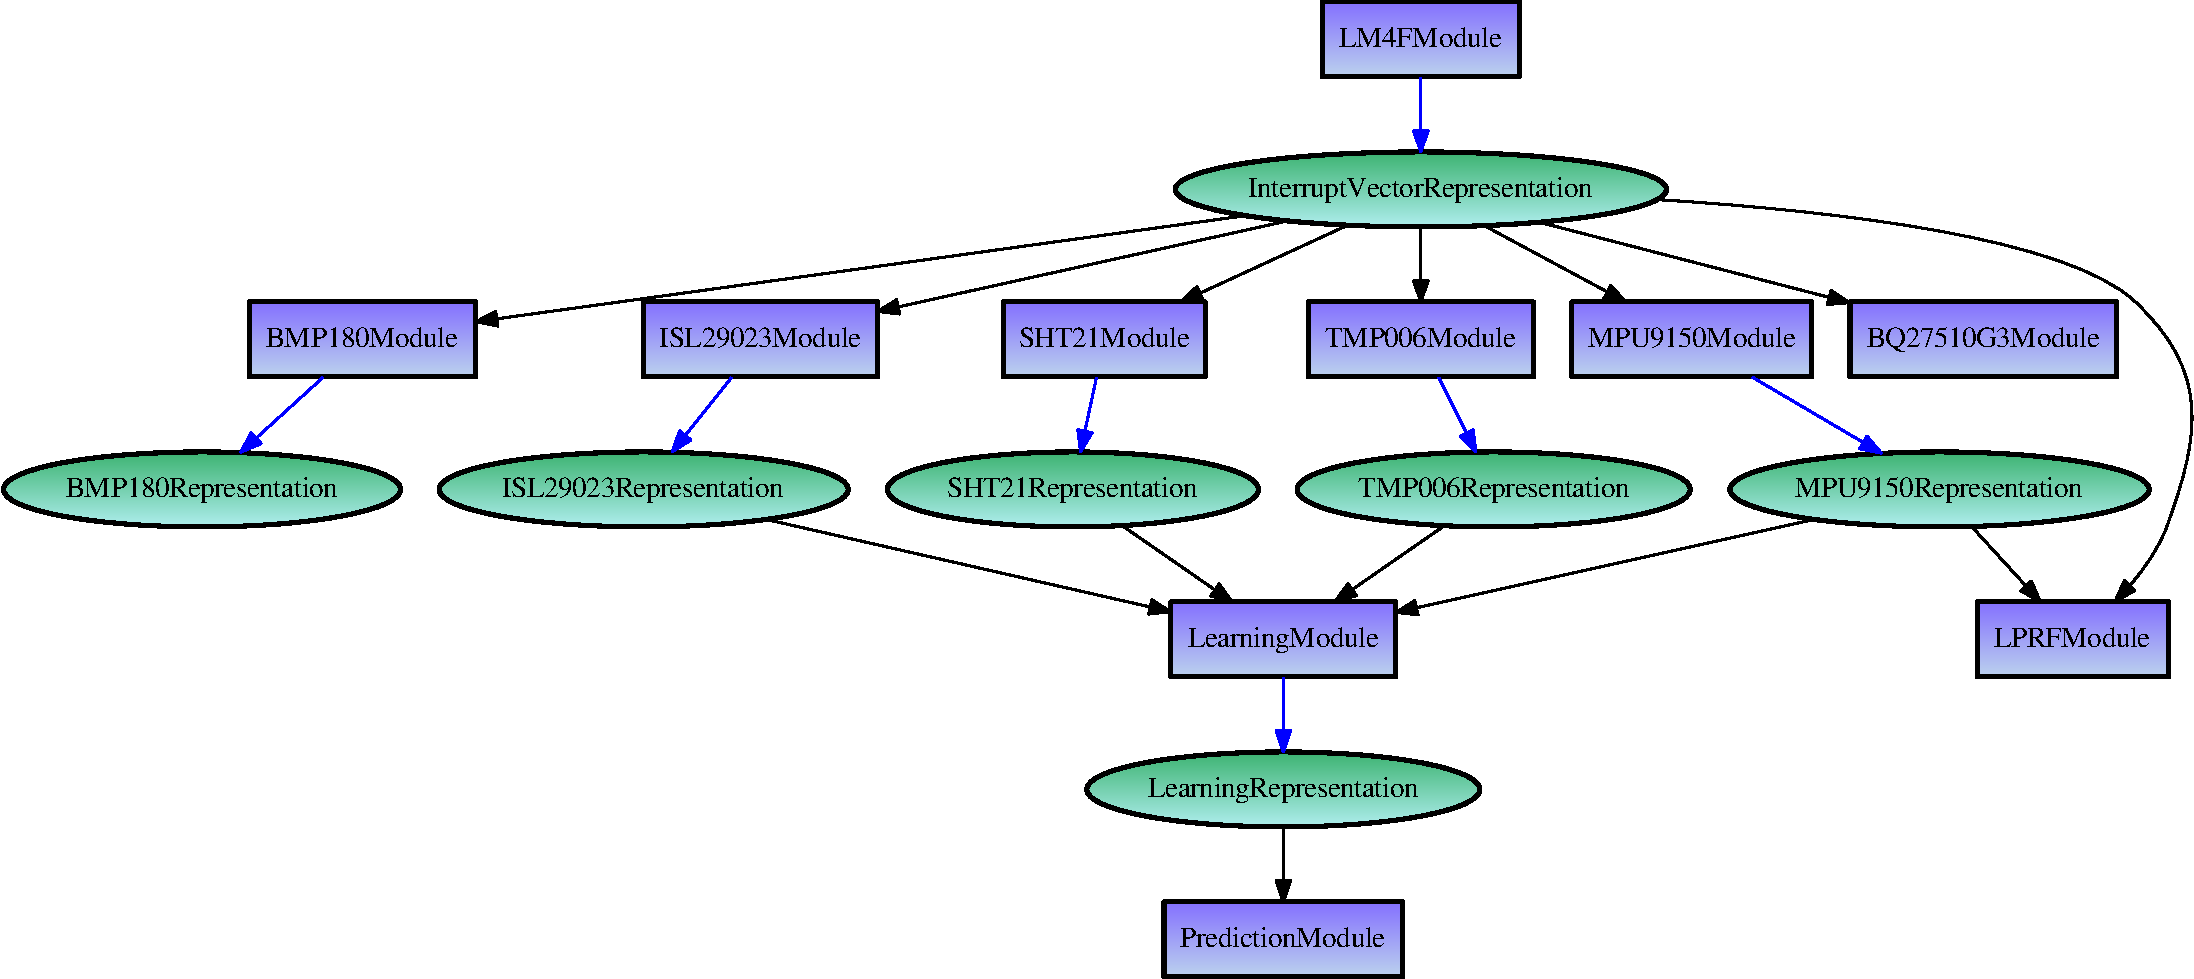
\includegraphics[width=0.57\textwidth]{figures/graph_structure_def-crop}} 
\subfloat[]{\label{fig:fb}\includegraphics[width=0.21\textwidth]{figures/human_figure}}
\subfloat[]{\label{fig:fc}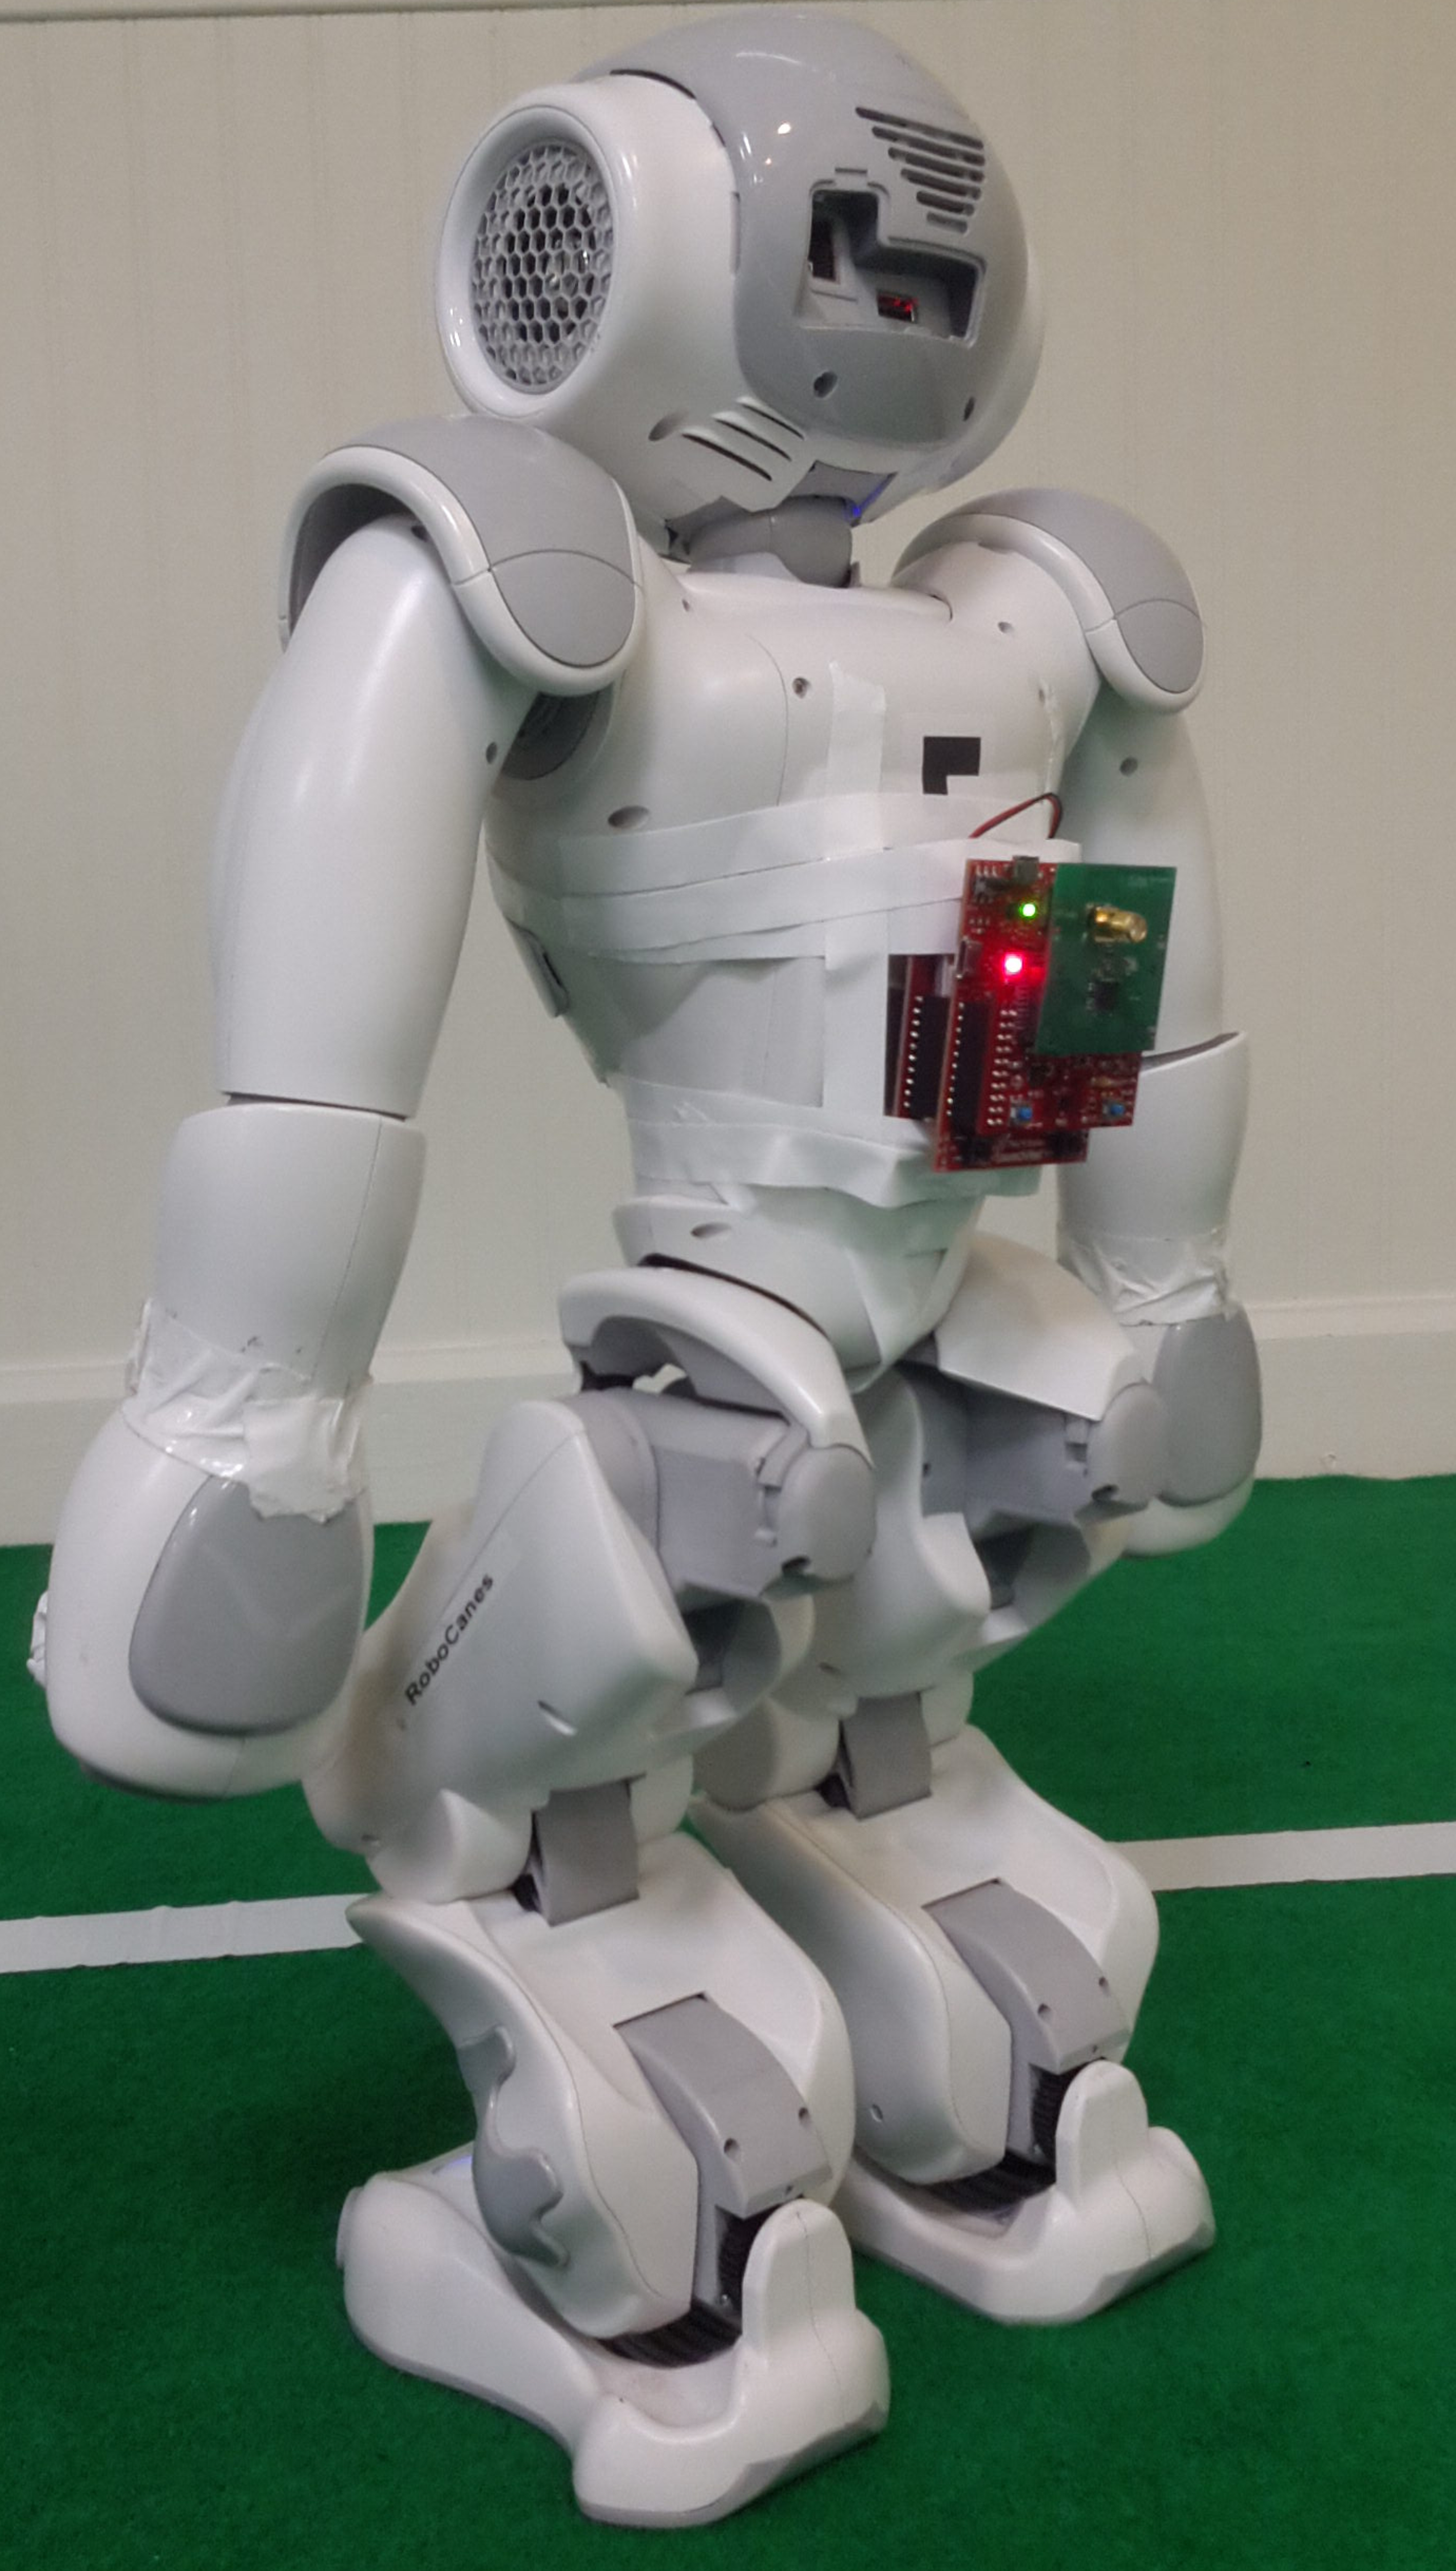
\includegraphics[width=0.185\textwidth]{figures/robot_figure}} 
\caption{(a) The modules and representations used in the experiments;  (b) the wireless radio was 
attached to a Sensor Hub BoosterPack on a Tiva C LaunchPad microcontroller that was connected to a 
Fuel Tank BoosterPack, which was then attached to the back of a human subject; and (c) the same 
device configuration was used on the back of a NAO humanoid robot.}
 \label{fig:framework}
\end{figure*}


%% added by faisal start
The existing activity detection methods focus on special cases of fall detection in humans and 
humanoid robots. These methods are primarily used in isolation.  
In SAFE (SmArt Fall dEtection) {~\cite{ojetola2011fall}} researchers used accelerometers and 
gyroscopes 
to detect fall incidence among the elderly people, they have used C4.5 decision tree to learn and 
classify fall and ADLs (activities of daily living). They claimed to identify four different types 
of falls with a precision of 81\% accuracy and recall of 92\% accuracy.
Javier Moya et. al.{~\cite{moya2014fall}} proposed a fall detection, avoidance and damage reduction 
mechanism for biped humanoid robots. They tried to simulate the real world environment where 
humanoid robots have to walk over irregular surface, running or playing sports, collusion with 
other 
robots and according to their article the proposed framework can detect instability and do fall 
avoidance or at least low-damage falling mechanism is invoked. 
%% faisal end

There has been an increasing interest in detecting human motions using embedded devices. Woon-Sung
et. al. \cite{baek2013real} proposed  a fall  detection  system  using necklace-shaped tri-axial
accelerometer  and  gyroscope  sensors  to  classify  the  behavior  and  posture  of  the detection
 subject. They claim that their  approach  can  successfully  distinguish between  ADL and  fall, 
with  sensitivities  greater  than  80 \%  and specificities  of  100\%. Ying-Wen et. al.
\cite{bai2013recognition} proposed an activity monitoring system based on smart phone sensor
reading and they claim that they can identify human activity with high degree of accuracy. Leno et.
al. \cite{leone2013supervised} prosed a system to detect event that cause trauma, and disabilities
using a tri-axial MEMS wearable wireless accelerometer. They have used support vector machine for
robust classification of different events. There has been similar efforts to detect human motions
using motion tracking, e.g., \cite{dumitrache2013fall,kumarwearable,liang2012pre}.


Compared to the existing solutions, we have provided a generalizable methods to detect human  and 
human-like activities from able-bodied humans and NAO humanoid robots. To our knowledge, we are the 
first to investigate the prospect of using an external embedded device to detect human-like motions 
on a NAO. The microcontrollers and embedded devices provide a flexible platform to 
build may real world applications. In order to build these applications, a practitioner would 
require  flexible and reliable software solutions. A practitioner also may require to use more than 
one functionality provided by the devices to build applications. Existing software solutions 
provide facilities to build applications to a certain degree, but, they lack methods or systems to 
integrate multiple devices simultaneously without much user burden. We have developed  
a state-of-the-art open source software solution to build heterogeneous applications on many 
devices, which can be programmed on multiple operating systems. 


Texas Instruments (TIs) microcontrollers\footnote{\url{https://www.ti.com/}} and add-on boards such 
as MSP430{\texttrademark}LaunchPad, Tiva{\texttrademark} C Series TM4C123G
LaunchPad (a low-cost evaluation platform for ARM Cortex-M4F-based microcontrollers), Tiva C Series 
TM4C129 Connected LaunchPad (a new development platform from Texas Instruments
based on the powerful TM4C129), and Sensor Hub BoosterPack (an add-on board designed to
fit Tiva C Series TM4C123G LaunchPad along with all of TI’s MCU LaunchPads) provide ultimate 
solutions for a wide rage of low power and portable applications. Therefore, a modular and flexible 
software framework allow practitioners to use the functionalities provides by these systems 
effectively and efficiently. The framework provides functionalities to build  rational agents that 
perceive its environment though sensors and act upon it though actuators \cite{russel2009}. The 
execution path between sensors to actuators may contain complex behaviors and modeling decisions 
that needs to be handled carefully. Hence, the framework takes these consideration into account and 
provides a topologically sorted graph based on the decision points provided by practitioners. Our
framework consists for four parts. It consists of modules and representations that execute on
\begin{inparaenum}[(1)]\item microcontrollers (incremental); \item offline (batch mode); \item NAO
robots; and \item real-time visualizations\end{inparaenum}. Our framework is lightweight, flexible, 
and consumes minimum memory and computational resources as possible. We have tested our framework on 
multiple microcontrollers and on a sensor hub as stated above. We have written and distributed 
software solutions to access devices on the sensor hub such as \begin{inparaenum}[(1)] \item 
InvenSense MPU-9150: 9-axis MEMS motion tracking (3-axis gyro 3-axis accelerometer, and 3-axis 
compass); \item Bosch Sensortec BMP180 pressure sensor; \item Sensirion SHT21 humidity and ambient 
temperature sensor; \item Intersil ISL29023 ambient and infrared light sensor; and \item TIs TMP006 
non-contact infrared temperature sensor\end{inparaenum}.

We have used our framework to experiment on the problem of activity
detection using InvenSense MPU-9150: 9-axis MEMS motion tracking sensor. We have conducted our
experiments on able-bodied humans and on NAO humanoid robots to detect activities such as standing,
walking, and abruptly falling back and front. We have used reactive (e.g., threshold based) 
and deliberative (e.g., machine learning) methods to detect these events and provide empirical  
justifications the success of the success of the methods. 


\section{Framework}

Our development framework\footnote{The library link has been anonymized.} uses a 
notion of 
{\em modules} and {\em representations} to perform
computations. The modules implement functions, while the representations exchange information from
one module to another. Figure \ref{fig:fa} shows the modules and representations related to our 
experiments. The boxes represent modules, while the ellipses represent the representations. As an
example, the module {\em MPU9150Module} contains logic to read/write from MPU-9150 Nine-Axis
(Gyro+Accelerometer+Compass) MEMS MotionTracking device on the sensor hub booster
pack. The representation {\em MPU9150Representation} contains all the values that the module
{\em MPU9150Module} would like to share with other modules. In this graph, {\em LearningModule}
requests values from {\em MPU9150Representation} to implement the learning function. A module can 
provide multiple representations. The blue arraws shows the provided representations, and the black 
arraws show the requested representations. The developers only require to write 
modules and representations, while the framework will compute the topologically sorted graph out of 
the nodes. This will be computed once, and the nodes in the queue will be executed one after the 
other. If there were to be cycles in the graph, the framework will detect them and indicate them to 
the developers.


\section{Approach and Evaluation}

\begin{figure*}[!t]
\centering
\subfloat[]{\label{fig:ha}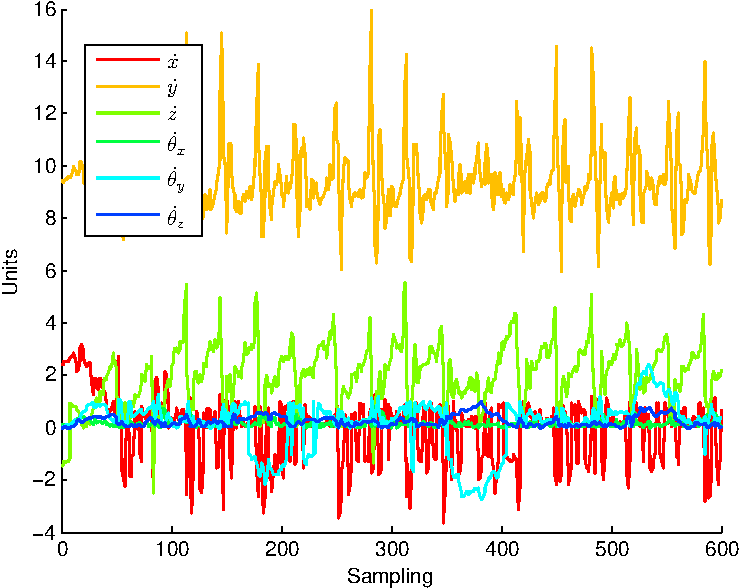
\includegraphics[width=0.33\textwidth]{plots/human_walk-crop.pdf}} 
\subfloat[]{\label{fig:hb}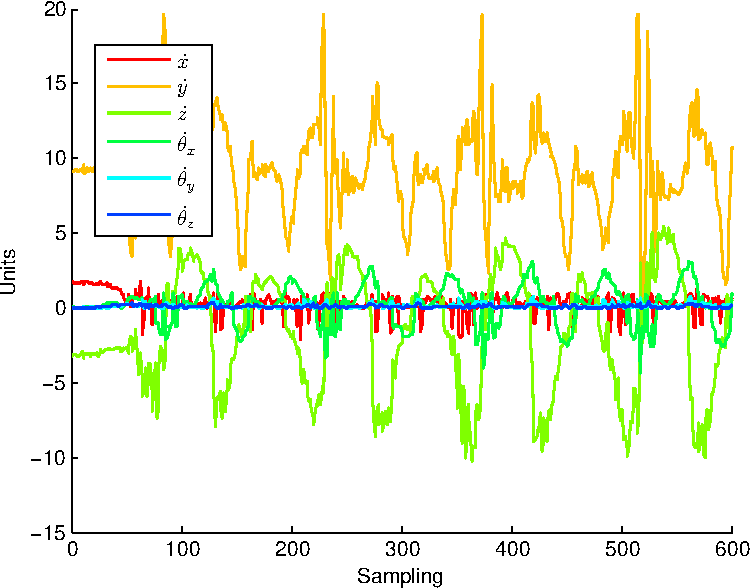
\includegraphics[width=0.33\textwidth]{plots/human_stand-crop.pdf}}
\subfloat[]{\label{fig:hc}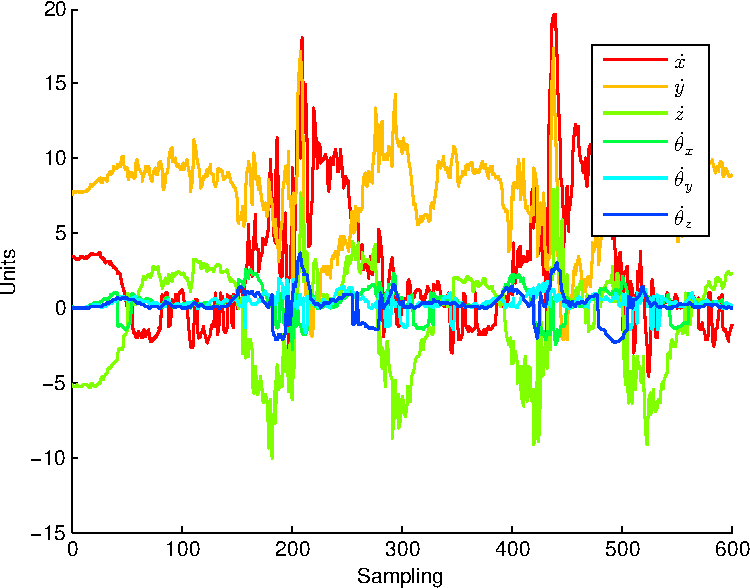
\includegraphics[width=0.33\textwidth]{plots/human_falling-crop.pdf}} 
\caption{~}
 \label{fig:human}
\end{figure*}


We have conducted experiments on detecting motions (activities) on able-bodied humans and on NAO
humanoid robots. In order to detect motions, we have used InvenSense MPU-9150: 9-axis MEMS
motion tracking sensor on the sensor hub. The module {\em MPU9150Module} connects to this device
and provides the representation {\em MPU9150Representation}. The representation contains
3-axis accelerometer readings, 3-axis gyroscope readings, 3-axis magnetometer readings, quaternion
rotation axis of the device, and Euler angles roll, pitch, and yaw.  In order to calculate Euler
angles, we have used the Direction Cosine Matrix (DCM)
algorithm.  Depending on the
experiment, the practitioner can change the sampling rate of the sensor.  The maximum sampling rate
of the sensor is 1000$Hz$. This section shows our results, validations, and conclusions.


\subsection{Falls annotation}
\textbf{to do need to change}
The annotation for a single fall event is shown in \textbf{{set the figure} }. The time for a 
complete protocol takes an average of ....... mins
per subject, and the time annotation per fall is about 5s. From
the figure, the area annotated as a fall is from 850s to 855s.
This shows that from point A to point B, the subject has been
instructed to fall and in the process of falling. Between points
B and C the subject’s body makes an impact with the cushion
on the floor and a high acceleration data is recorded. After a
fall has occurred, the subject remains in a lying posture at point
C to D. Though, point A to D was annotated as a fall, only
point B to C shows a high acceleration signal. The following
section discusses the data processing, machine learning and
the results obtained
\textbf{to do need to change}


\subsection{Able-Bodied Human}

We have collected data for different human activities. We have put the sensors on the back of the
human body and collected data from those sensors in fixed interval. For this experiment, we have
sampled data in 50$Hz$ (or 20$ms$). We have data from several different human configurations:
\begin{inparaenum}[(1)] \item standing; \item seating; \item walking; \item standing to seating;
and \item standing to falling\end{inparaenum}. We have collected data based on the activities and
each data point has nine features, where three sensors accelerometers,gyroscope and magnetometers have three axis X, Y and Z.

\par
A falling event does not happen within a single reading from sensors, it is consists of multiple
reading from sensors.  Its not really accurate to detect a fall or any other motion based on a
single reading, which might mislead the whole detection procedure. To detect a motion accurately we
have used a time frame based prediction procedure. In this procedure, we first train our SVM with
training data. Then we try to detection motion in each sensor reading. We will predict a motion not
based on a single reading but with all the reading within 200$ms$ time frame. If our detection
procedure detect a true fall event more than 90\% time, we will denote that event as a true
falling event.

\subsection{Classification using Logistic Regression}

In the first part of the data analysis we have put all our collected data together and labeled it
with specific number to denote the position. We have used multivariate logistic regression model to
classify our data. We have used 80\% of the data for training, while the rest has been used
in validation.


\begin{table}[!ht]
\caption{Logistic regression Classification}
	\label{tab:human-logistic-class}
	\centering
		\begin{tabular} {|l |c |c |c|c|}
			\hline
			{\bf Activity} & {\bf  TP}  &	{\bf TN}  &	{\bf FP} &	{\bf FN} \\ 
			\hline
			Walking	& 88\%	& 84\%	& 16\%	& 12\% \\ \hline
			Stand to seat	& 92\%	& 82\%	& 18\% & 	8\%	 \\ \hline 
			Stand to fall	& 92\%	& 88\%	& 12\%	& 8\%	 \\ \hline
		\end{tabular}
\end{table}




\subsection{Classification and Validation using Support Vector Machine}

In the second part of the data analysis, we have used support vector machine (SVM) model
to classify our data. To train the model, we used the same procedure as before, 80\% of
our data were used to do the classification and rest twenty percent data were used to validate our
classification result.




\begin{table}[!ht]
\caption{SVM Classification}
	\label{tab:human-svm-class}
	\centering
		\begin{tabular} {|l |c |c |c|c|}
			\hline
			{\bf Activity} & {\bf  TP}  &	{\bf TN}  &	{\bf FP} &	{\bf FN} \\ 
			\hline
			Walking	& 92\%	& 86\%	& 14\%	& 8\% \\ \hline
			Stand to seat	& 94\%	& 84\%	& 16\% & 	6\%	 \\ \hline 
			Stand to fall	& 98\%	& 88\%	& 12\%	& 2\%	 \\ \hline
		\end{tabular}
\end{table}

\subsection{NAO Humanoid Robot}


We have used the device configuration as described  in the subsection {\em Able-Bodied Human} 
and it was attached to the robot as shown in Figure \ref{fig:fc}. We have also followed the same 
data collection protocol. In the first experiment, we have designed a thresholding base activity 
predictor. We have calculated the roll, pitch, and yaw angles for this study (the roll is around 
x-axis, the pitch is around y-axis, and the yaw is around z-axis). We have configured InvenSense 
MPU-9150: 9-axis MEMS motion sensor on the sensor hub to sample data
at 50$Hz$. We have chosen this value to compensate delays in communications and to cope with the
constraints provided by the robot. In this study, we have detected only the normal 
activities (marching, waling forward/backward, and turning clockwise/counter-clockwise)
and falling activities (falling back, front, and sideways). 

\begin{figure*}[!ht]
  \centering
  \subfloat[Marching in place.]{\label{fig:tsnedataset_1}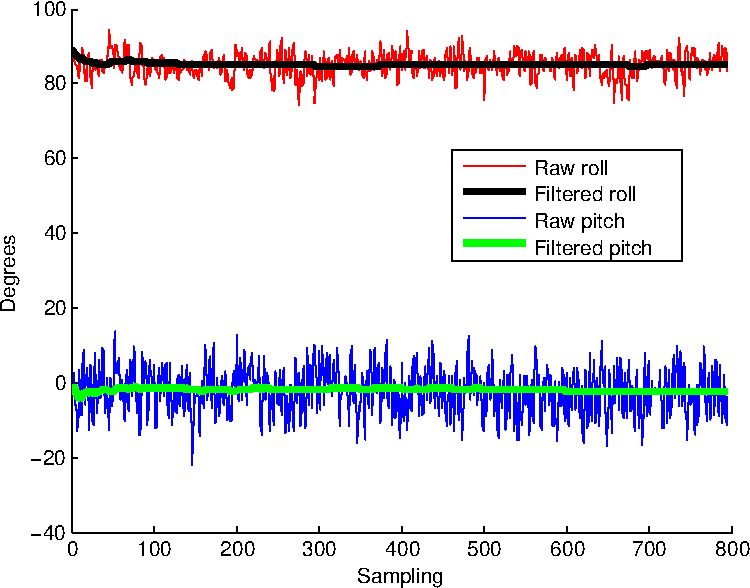
\includegraphics[width=0.25\textwidth]
       {plot1-crop}} 
  \subfloat[Walking backward.]{\label{fig:tsnedataset_9}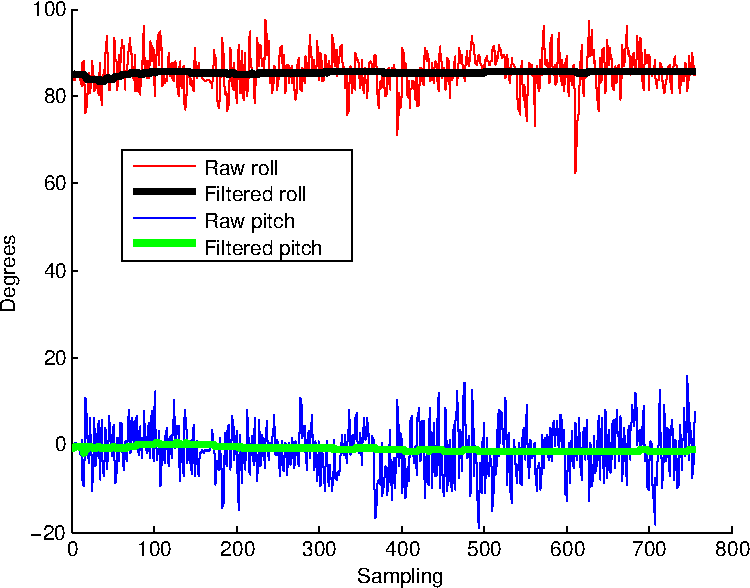
\includegraphics[width=0.25\textwidth]
       {plot5-crop}}
  \subfloat[Rotating clockwise.]{\label{fig:tsnedataset_7}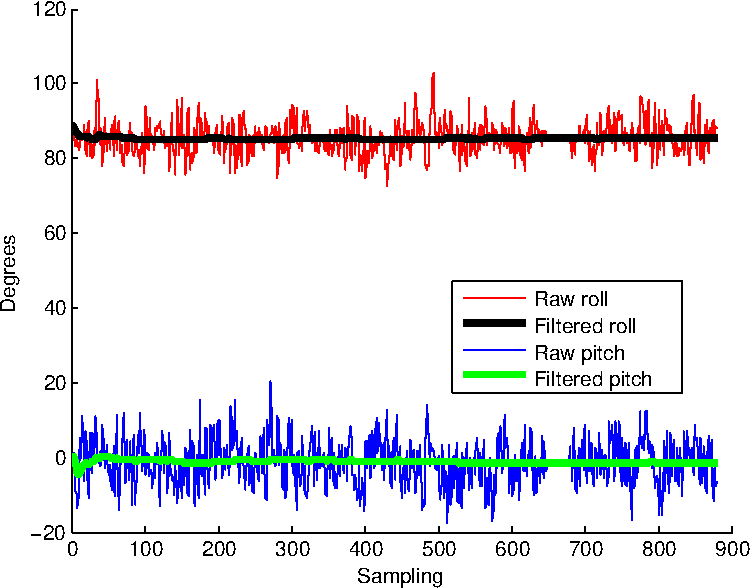
\includegraphics[width=0.25\textwidth]
       {plot2-crop}}
  \subfloat[Left side-way walk.]{\label{fig:tsnedataset_10}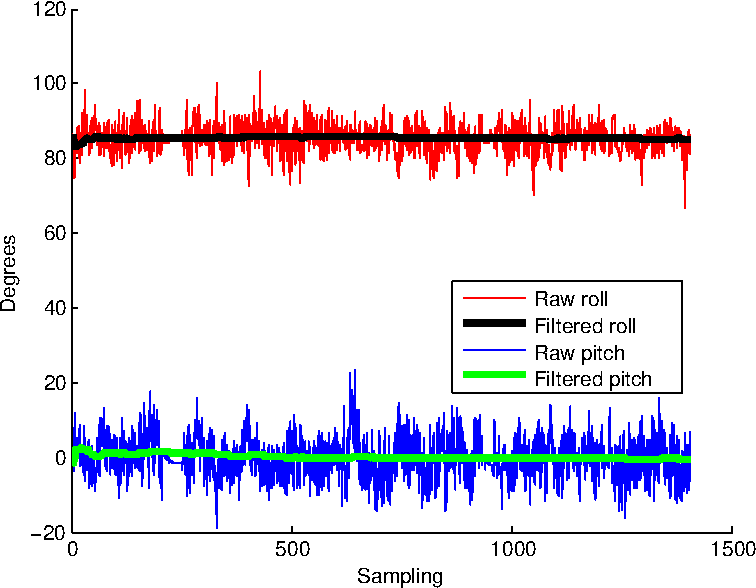
\includegraphics[width=0.25\textwidth]
       {plot6-crop}}
       \\
  \subfloat[Falling forward.]{\label{fig:tsnedataset_11}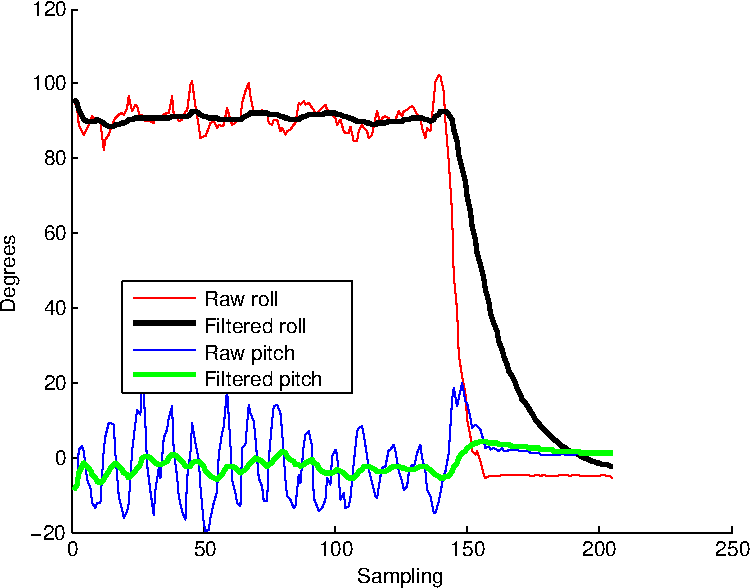
\includegraphics[width=0.25\textwidth]
       {plot1_fallen-crop}}
  \subfloat[Falling backward.]{\label{fig:tsnedataset_12}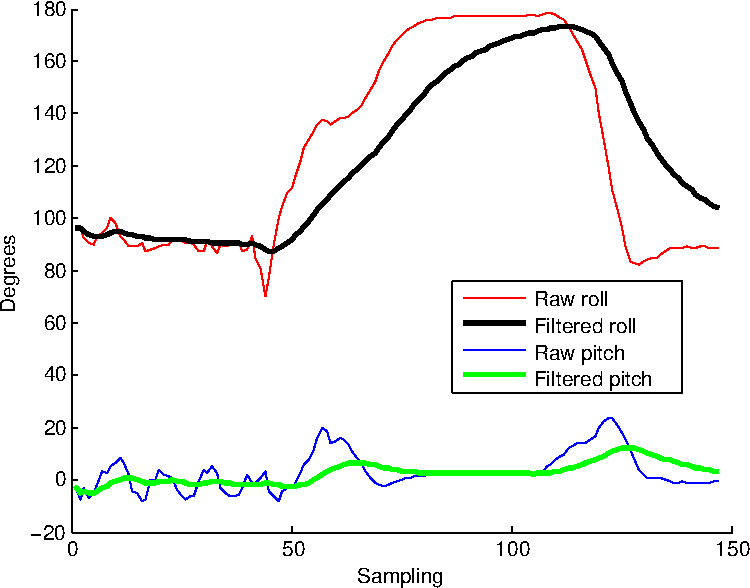
\includegraphics[width=0.25\textwidth]
       {plot2_fallen-crop}}
  \subfloat[Falling to left side.]{\label{fig:tsnedataset_13}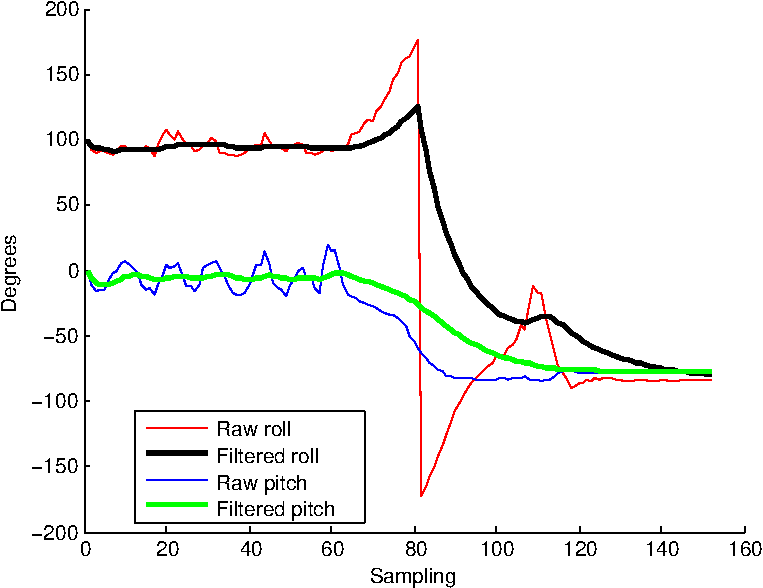
\includegraphics[width=0.25\textwidth]
       {plot3_fallen-crop}}
  \subfloat[Falling to right
side.]{\label{fig:tsnedataset_14}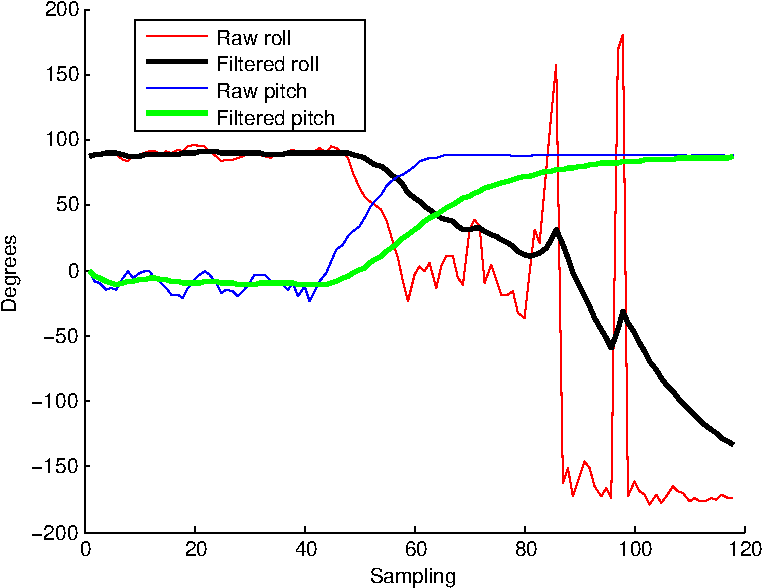
\includegraphics[width=0.25\textwidth]
       {plot4_fallen-crop}}      
  \caption{Figures (a)-(d) show the roll and pitch angles (raw and filtered) for normal 
behavior. Figures (e)-(h) show the raw and filtered roll and pitch angles for fallen 
states of NAO humanoid robot.}
  \label{fig:normalFallenBehavior}

\end{figure*}

Our NAO humanoid robots have omni-directional walking engines to conducts primary  
movements. These movements are regulated by linear velocities $\dot{x}_v$ and $\dot{y}_v$, and a 
angular velocity $\dot{\theta}_v$ input parameters. Depending on these
values, we can let the robot walk (forward, backward, and side-ways), and rotate (clockwise and
counter-clockwise) with different speeds. In this study, we have considered \begin{inparaenum}[(1)]
\item marching ($\dot{x}_v = 0 , \dot{y}_v = 0, \dot{\theta}_v = 0$); \item walking  
forward/backward ($\dot{x}_v = \pm200
, \dot{y}_v = 0, \dot{\theta}_v = 0$);  \item walking side-ways ($\dot{x}_v = 0, \dot{y}_v = 
\pm200, \dot{\theta}_v = 0$); and  \item rotating clockwise/counter-clockwise
($\dot{x}_v = 0 , \dot{y}_v = 0, \dot{\theta}_v = \pm 0.5$) \end{inparaenum} as {\em normal state}, 
while, all the other activities have been classified as {\em fallen state}. 

\begin{table}[!ht]
\caption{Logistic regression Classification}
	\label{tab:robot-logistic-class}
	\centering
		\begin{tabular} {| l | c | c | c| c|}
		\hline
			{\bf Activity} & {\bf  TP}  &	{\bf TN}  &	{\bf FP} &	{\bf FN} \\ 
\hline
			Walking forward	& 86\%	& 84\%	& 16\%	& 14\% \\ \hline
			Walking backward	& 86\%	& 84\%	& 16\%	& 14\% \\ \hline
			Walking left 	& 88\%	& 86\%	& 14\%	& 12\% \\ \hline
			Walking right 	& 86\%	& 84\%	& 16\%	& 14\% \\ \hline
			Falling forward	& 94\%	& 90\%	& 10\%	& 6\%	 \\ \hline
			Falling Backward	& 94\%	& 88\%	& 12\%	& 6\%	 \\ \hline
			Falling left	& 92\%	& 92\%	& 8\%	& 8\%	 \\ \hline
			Falling Right	& 92\%	& 92\%	& 8\%	& 8\%	 \\ \hline
			Marching	& 88\%	& 84\%	& 16\%	& 12\%	 \\ \hline
			Rotate CCW	& 94\%	& 90\%	& 10\%	& 6\%	 \\ \hline
			Rotate CW	& 94\%	& 90\%	& 10\%	& 6\%	 \\ \hline
		\end{tabular}
\end{table}


We have used only the roll and the pitch values  to detect relevant activities. In order to achieve 
an effective threshold based decision making, first we have filtered the roll, pitch, and
yaw values using a Kalman filter \cite{Welch:1995:IKF:897831}. Figures 
\ref{fig:normalFallenBehavior} ((a)--(d)) show
the raw and the filtered values of the raw and the pitch values for marching, walk backward,
rotating clockwise, and left side-way walk. The other activities show similar plots (we have 
refrained from plotting them due to space constraints). The thresholding method
suggests that, if the filtered roll values are within the range $[90\pm15]$ (degrees) and the
filtered pitch values are within the rage $[0\pm15]$ (degrees), then with 100\% accuracy, NAO 
humanoid robot will is in a normal state. Otherwise, we can safely assume that the robot is in 
a fallen state.   

We have defined four fallen states for the robot: \begin{inparaenum}[(1)] \item falling
forward; \item falling backward; \item falling to left side; and \item falling to right
side\end{inparaenum}. Figures \ref{fig:normalFallenBehavior} ((e)--(h)) show the roll and pitch 
angles (raw and filtered) for typical fallen robot. If the filtered roll value is less that 60 
degrees, we can safely assume that the robot is falling forward. If the filtered roll values is 
more than 100 degrees we can assume that the robot is falling backward. To detect the events 
falling to the left and right, we have used the filtered pitch values. If the filtered pitch value 
is less than -50 degrees, we can assume that the robot is falling to the left side, while if the 
filtered pitch values is more than 50 degrees, we can assume that the robot is falling to the right 
side. With these thresholds for a separate test cases, the thresholding method has detected fallen 
state with 100\% accuracy. 


Even though thresholding method successfully distinguished between normal and fallen states, it was 
unable to detect states within normal activities, i.e., walking forward to waling backward so 
forth. Therefore, similar to the previous experiments, we have used logistic regression and SVM 
classifiers to identify different activities. FixMe:


\begin{table}[!ht]
\caption{SVM Classification}
	\label{tab:robot-svm-class}
	\centering
		\begin{tabular} {| l | c | c | c | c | }
		\hline
			{\bf Activity} & {\bf  TP}  &	{\bf TN}  &	{\bf FP} &	{\bf FN} \\ 
\hline
			Walking forward	& 90\%	& 88\%	& 12\%	& 10\% \\ \hline
			Walking backward	& 90\%	& 88\%	& 12\%	& 10\% \\ \hline
			Walking left	& 92\%	& 86\%	& 14\%	& 8\% \\ \hline
			Walking right	& 92\%	& 86\%	& 14\%	& 8\% \\ \hline
			Falling forward	& 96\%	& 90\%	& 10\%	& 4\%	 \\ \hline
			Falling backward	& 96\%	& 88\%	& 12\%	& 4\%	 \\ \hline
			Falling left	& 94\%	& 92\%	& 8\%	& 6\%	 \\ \hline
			Falling right	& 94\%	& 92\%	& 8\%	& 6\%	 \\ \hline
			Marching	& 90\%	& 88\%	& 12\%	& 10\%	 \\ \hline
			Rotate CCW	& 96\%	& 90\%	& 10\%	& 4\%	 \\ \hline
			Rotate CW	& 96\%	& 90\%	& 10\%	& 4\%	 \\ \hline
		\end{tabular}
\end{table}

The range of motion of NAO humanoid robot is comparatively constrained compared to a able-bodied 
human. Therefore, we only conduct primary activities as described in this section. We have not 
conducted experiments on activities such as stand to seat. When determining the results, we 
have sampled the motion device data at the rate 50$Hz$. During operation, if using the 
thresholding method, we can use the same thresholds, with higher sampling rate. The second method 
requires learning for different sampling rates. 





\section{Conclusion and Future Work}

In this project, we have proposed an open source software solution to write heterogeneous
applications on TIs microcontrollers. We have used our software solution to detect motions on
able-bodied humans and NAO humanoid robots. We have shown that our methods are capable of detecting
motions with high accuracy. We have used machine learning methods and thresholding methods to
detect different motions and provided justifications for the success of the applications. 

\par
Comparing the encouraging experimental results achieved, our future work will be c

\bibliographystyle{aaai}
\bibliography{references}


\end{document}
